\documentclass[aspectratio=169]{beamer}

\usepackage{amsmath}
\usepackage{amssymb}
\usepackage{symbols}
\usepackage{caption}
\usepackage{subcaption}
\usepackage{tabularray}
\usepackage{makecell}
\usepackage{tikz}
\usepackage{lmodern}
\usepackage[ruled,vlined,noend]{algorithm2e}
\usepackage{pgfpages}
\usepackage{listings}
\usepackage{xcolor}
\usepackage{appendixnumberbeamer}

\lstdefinestyle{pythonstyle}{
    language=Python,
    basicstyle=\ttfamily\footnotesize,
    keywordstyle=\color{blue}\bfseries,
    commentstyle=\color{green!50!black},
    stringstyle=\color{red},
    showstringspaces=false,
    breaklines=true,
    numberstyle=\tiny\color{gray},
    xleftmargin=0.5em,
    framexleftmargin=0.5em
}

\definecolor{darkpurple}{RGB}{142,20,242}
\hypersetup{colorlinks,linkcolor=,urlcolor=blue}
\usecolortheme{beaver}
\setbeamercolor{frametitle}{fg=white,bg=darkpurple}
\setbeamercolor{title}{fg=white,bg=darkpurple}
\setbeamercolor{structure}{fg=darkpurple}
\setbeamercolor{itemize item}{fg=darkpurple}
\setbeamercolor{itemize subitem}{fg=darkpurple}
\setbeamercovered{invisible}
\setlength{\parskip}{3.5ex}
\setbeamertemplate{footline}[frame number]
\beamertemplatenavigationsymbolsempty

\title{TorchJD: Jacobian Descent in PyTorch}
\date{
\includegraphics[height=2.2cm]{images/pytorch-eu}}

\author{%
  \hspace{0.35cm}Val\'erian Rey --- \texorpdfstring{\texttt{valerian.rey@gmail.com}}{valerian.rey@gmail.com}\texorpdfstring{\\}{ - }%
  Pierre Quinton --- \texorpdfstring{\texttt{pierre.quinton@epfl.ch}}{pierre.quinton@epfl.ch}\texorpdfstring{\\}{ - }%
}

\begin{document}

\begin{frame}[plain, noframenumbering]
\maketitle
\tikz[remember picture, overlay] {
  % Left: GitHub
  \node[anchor=south west, inner sep=0pt] at ([xshift=0.5cm, yshift=0.5cm]current page.south west) {
    \begin{minipage}{4cm}
      \raggedright
      
\includegraphics[width=1.4cm]{images/logos/github}\\
      \href{https://github.com/SimplexLab/TorchJD}{\small github.com/SimplexLab/TorchJD}
    \end{minipage}
  };
  % Center: Documentation
  \node[anchor=south, inner sep=0pt] at ([yshift=0.5cm]current page.south) {
    \begin{minipage}{4cm}
      \centering
      
\includegraphics[width=2.1cm]{images/logos/torchjd2}\\
      \href{https://torchjd.org/}{\small torchjd.org}
    \end{minipage}
  };
  % Right: ArXiv
  \node[anchor=south east, inner sep=0pt] at ([xshift=-0.5cm, yshift=0.5cm]current page.south east) {
    \begin{minipage}{4cm}
      \raggedleft
      
\includegraphics[width=1.4cm]{images/logos/arxiv}\\
      \href{https://arxiv.org/pdf/2406.16232}{\small arxiv.org/pdf/2406.16232}
    \end{minipage}
  };
}
\end{frame}

\begin{frame}[plain, noframenumbering]
\frametitle{Table of contents}
{\setlength{\parskip}{0pt}
\setbeamertemplate{section in toc}{~\textbf{\inserttocsection}}
\setbeamertemplate{subsection in toc}{\hspace{0.4cm}~\inserttocsubsection\par}
\tableofcontents}
\end{frame}

\section{Theory}

\begin{frame}
\centering
\Huge Theory
\end{frame}

\subsection{Unconflicting projection of gradients (UPGrad)}
\begin{frame}{Unconflicting projection of gradients (UPGrad)}

\only<1>{\tikz[remember picture, overlay] \node[yshift=-0.5cm] at (current page.center) {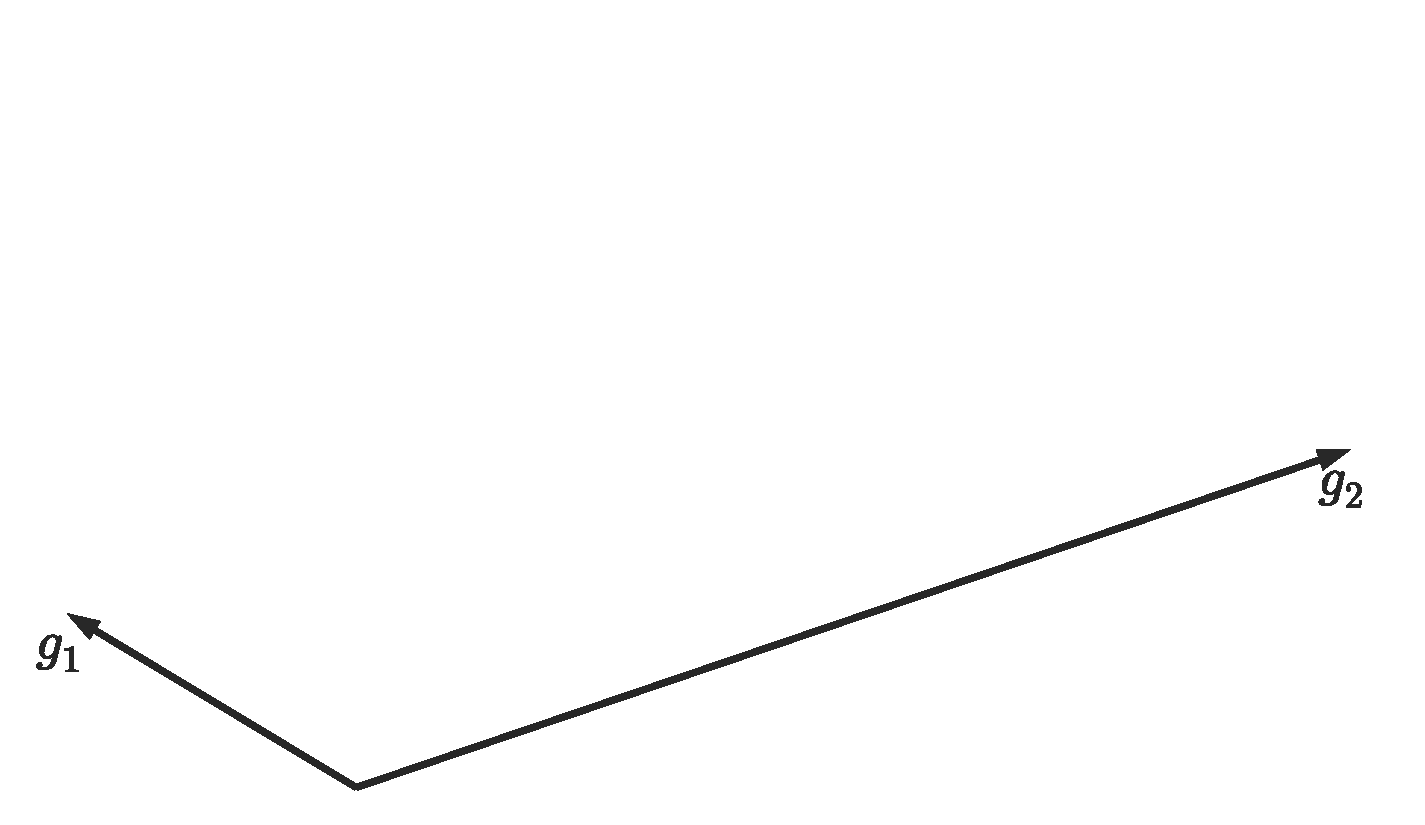
\includegraphics[width=10cm]{images/dual_cone/gradients}};}
\only<2>{\tikz[remember picture, overlay] \node[yshift=-0.5cm] at (current page.center) {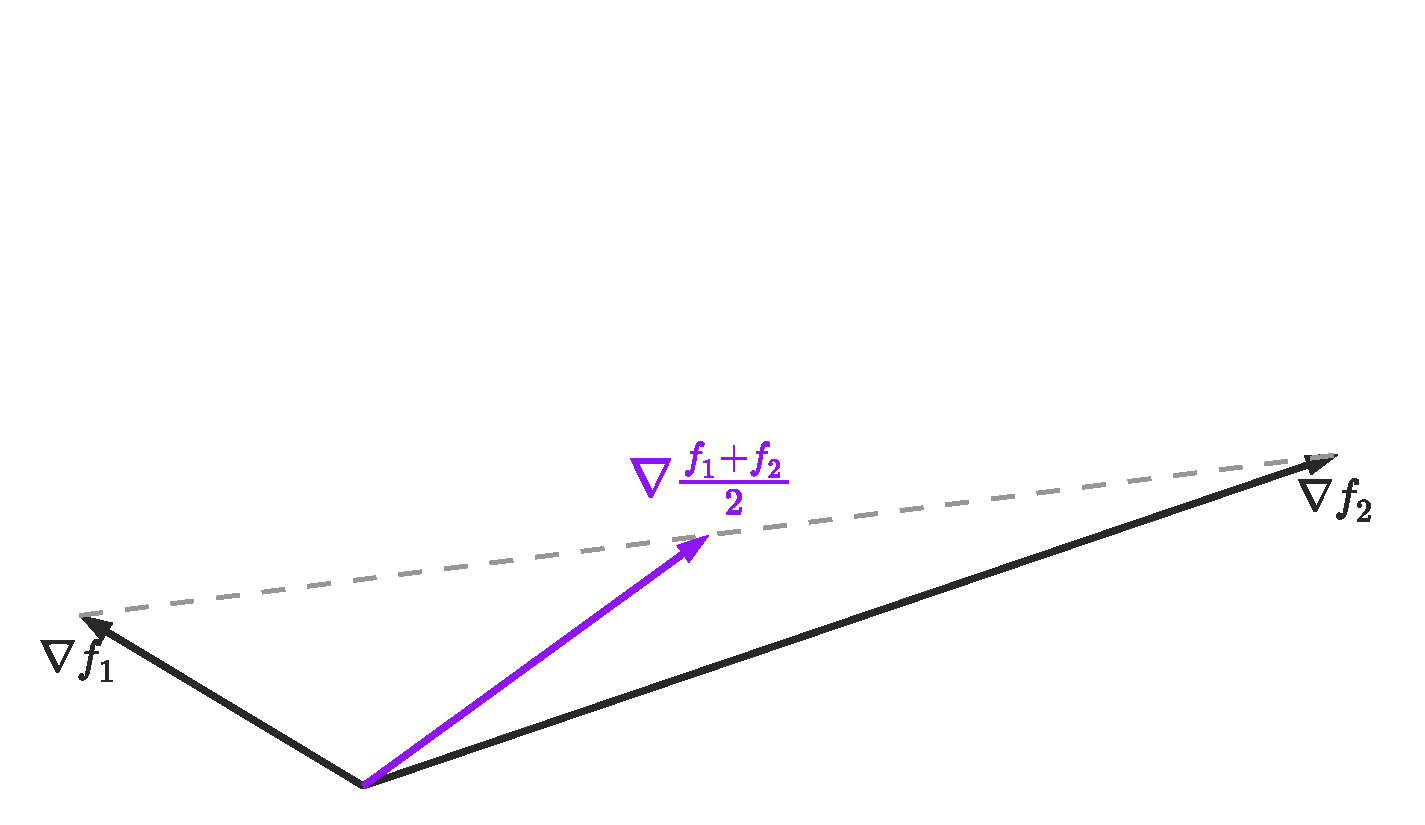
\includegraphics[width=10cm]{images/dual_cone/gradients_mean}};}
\only<3>{\tikz[remember picture, overlay] \node[yshift=-0.5cm] at (current page.center) {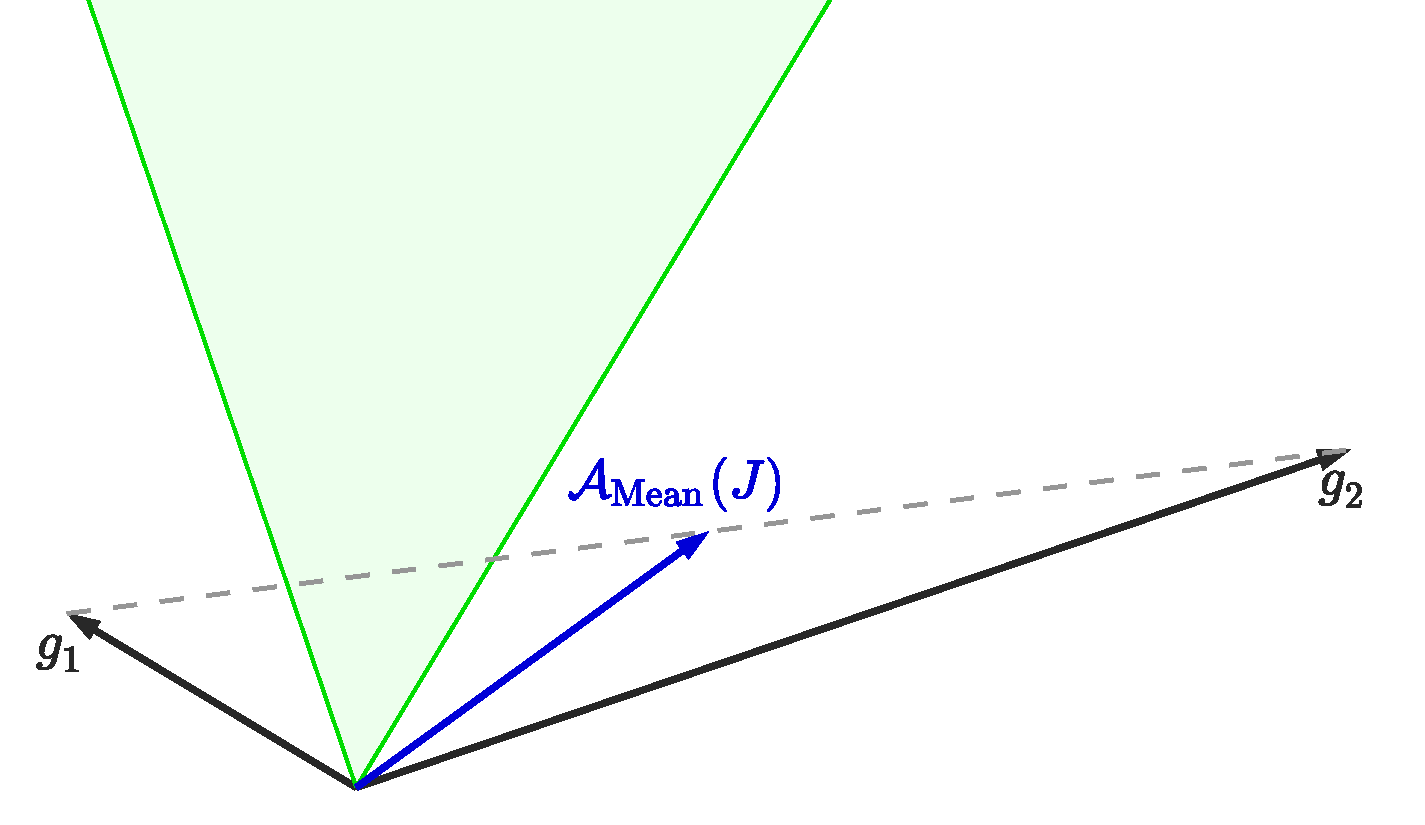
\includegraphics[width=10cm]{images/dual_cone/gradients_cone_mean}};}
\only<4>{\tikz[remember picture, overlay] \node[yshift=-0.5cm] at (current page.center) {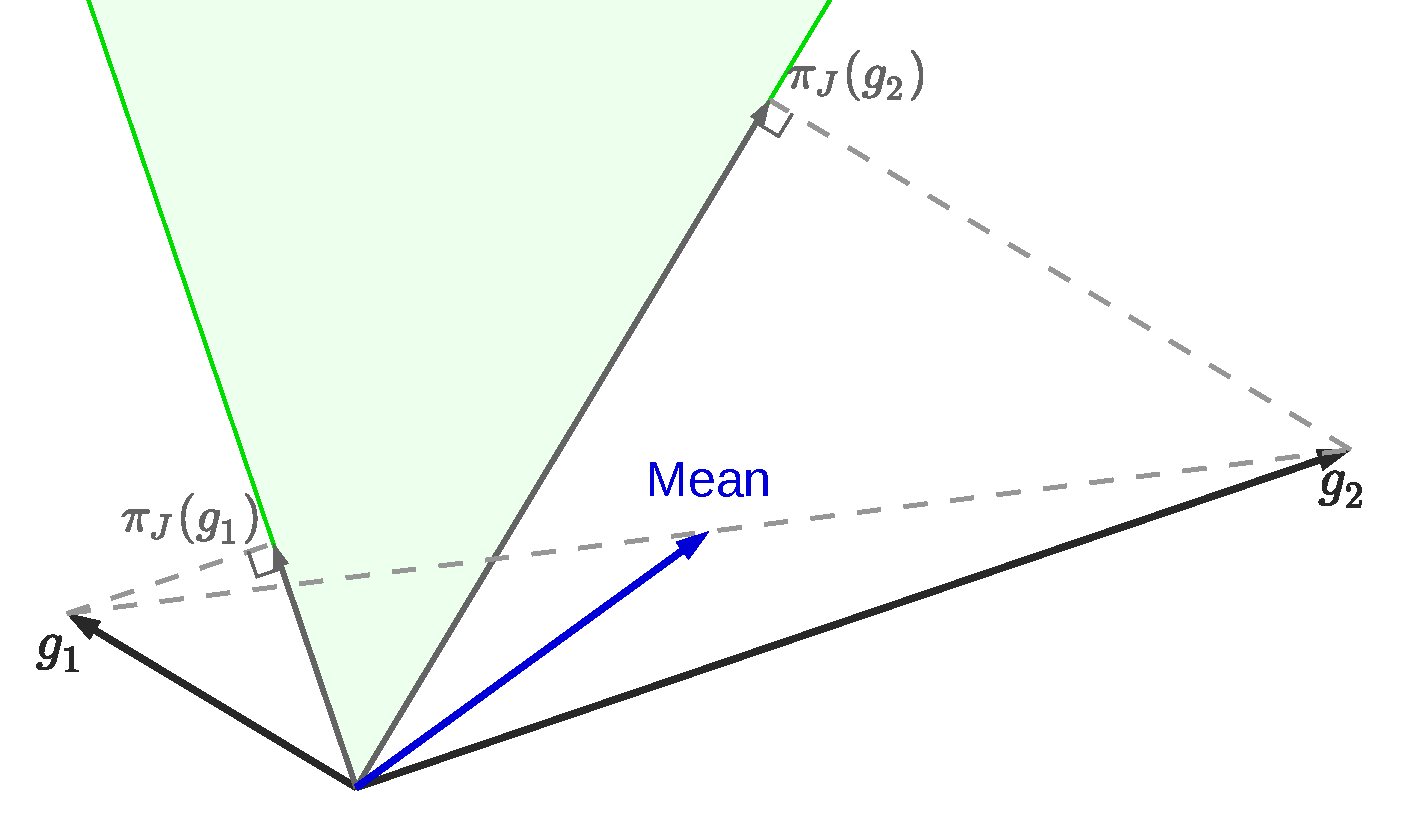
\includegraphics[width=10cm]{images/dual_cone/gradients_cone_projections_mean}};}
\only<5>{\tikz[remember picture, overlay] \node[yshift=-0.5cm] at (current page.center) {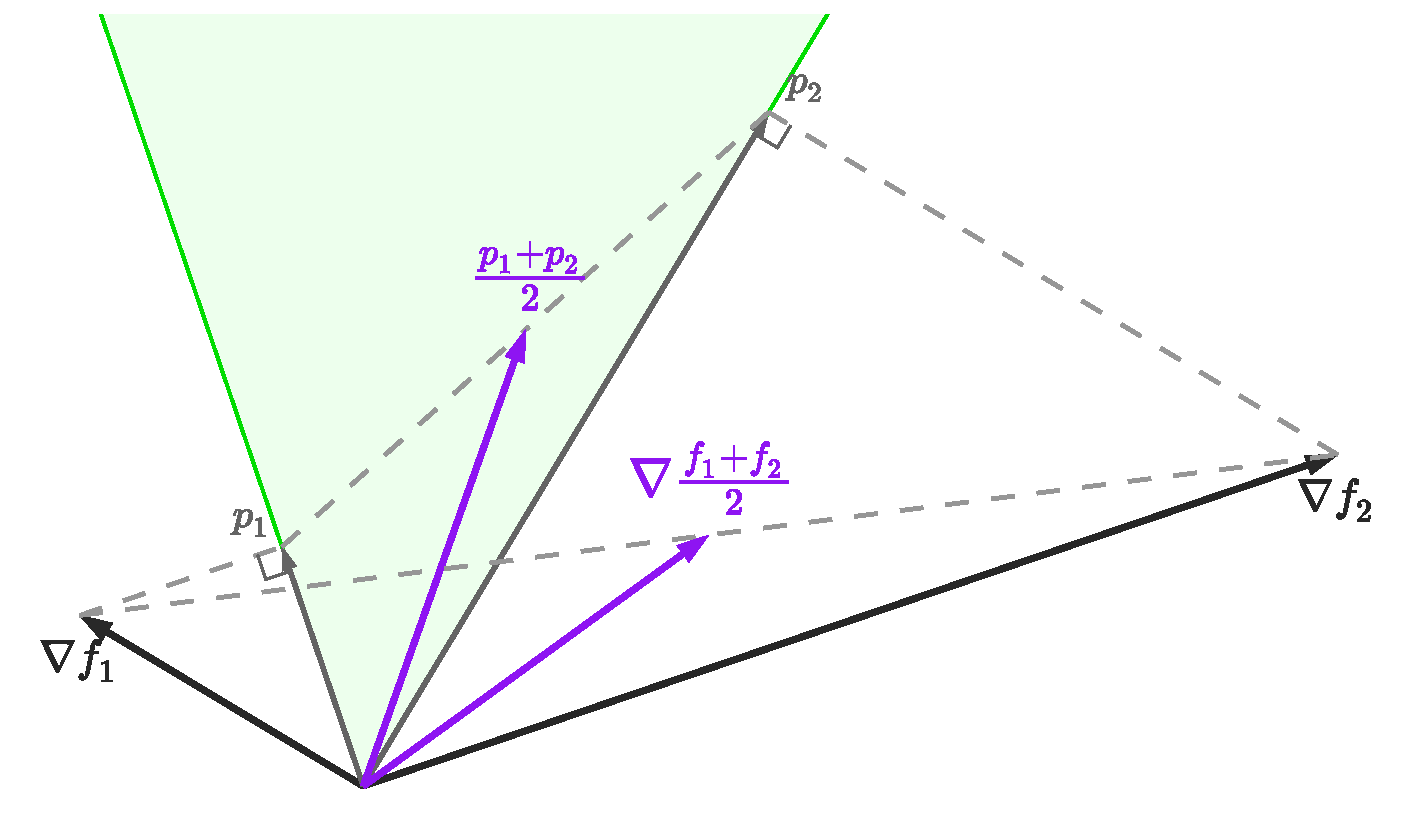
\includegraphics[width=10cm]{images/dual_cone/gradients_cone_projections_upgrad_mean}};}

\vspace{-4.3cm}
\hfill $J = \begin{bmatrix} g_1^\T \\ g_2^\T \end{bmatrix}$ \hspace{0.5cm}
\end{frame}

\section{Conclusion}
\begin{frame}{Conclusion}
Many problems are multi-objective.
\pause

TorchJD to compute and aggregate Jacobians.
\pause

Try to compute the inner products between your gradients.
\pause

Can JD solve problems that GD can't?
\end{frame}

\appendix

\begin{frame}
\centering
\Huge Appendix
\end{frame}

\end{document}
